% Graphic for TeX using PGF
% Title: /home/aleix/pfc_svn/doc/imatges/model/mtsdb-arquitecura_interna.en.dia
% Creator: Dia v0.97.1
% CreationDate: Mon Nov 14 13:03:36 2011
% For: aleix
% \usepackage{tikz}
% The following commands are not supported in PSTricks at present
% We define them conditionally, so when they are implemented,
% this pgf file will use them.
\ifx\du\undefined
  \newlength{\du}
\fi
\setlength{\du}{15\unitlength}
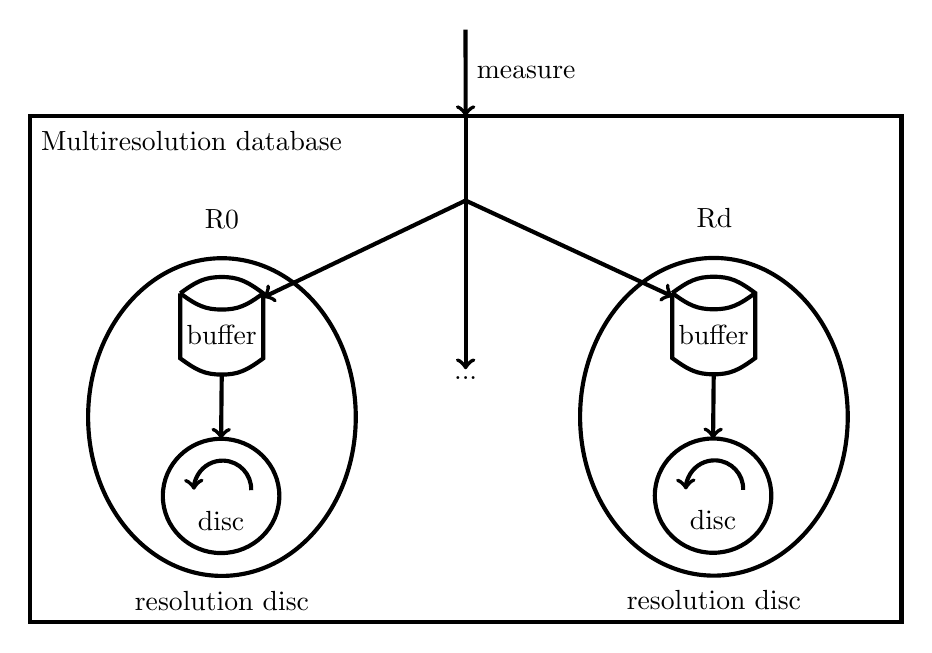
\begin{tikzpicture}
\pgftransformxscale{1.000000}
\pgftransformyscale{-1.000000}
\definecolor{dialinecolor}{rgb}{0.000000, 0.000000, 0.000000}
\pgfsetstrokecolor{dialinecolor}
\definecolor{dialinecolor}{rgb}{1.000000, 1.000000, 1.000000}
\pgfsetfillcolor{dialinecolor}
\definecolor{dialinecolor}{rgb}{1.000000, 1.000000, 1.000000}
\pgfsetfillcolor{dialinecolor}
\fill (7.137500\du,-8.100000\du)--(7.137500\du,4.093750\du)--(28.137500\du,4.093750\du)--(28.137500\du,-8.100000\du)--cycle;
\pgfsetlinewidth{0.100000\du}
\pgfsetdash{}{0pt}
\pgfsetdash{}{0pt}
\pgfsetmiterjoin
\definecolor{dialinecolor}{rgb}{0.000000, 0.000000, 0.000000}
\pgfsetstrokecolor{dialinecolor}
\draw (7.137500\du,-8.100000\du)--(7.137500\du,4.093750\du)--(28.137500\du,4.093750\du)--(28.137500\du,-8.100000\du)--cycle;
% setfont left to latex
\definecolor{dialinecolor}{rgb}{0.000000, 0.000000, 0.000000}
\pgfsetstrokecolor{dialinecolor}
\node at (17.637500\du,-1.808125\du){};
% setfont left to latex
\definecolor{dialinecolor}{rgb}{0.000000, 0.000000, 0.000000}
\pgfsetstrokecolor{dialinecolor}
\node at (17.637500\du,-1.781870\du){...};
% setfont left to latex
\definecolor{dialinecolor}{rgb}{0.000000, 0.000000, 0.000000}
\pgfsetstrokecolor{dialinecolor}
\node at (11.767300\du,-5.630860\du){R0};
% setfont left to latex
\definecolor{dialinecolor}{rgb}{0.000000, 0.000000, 0.000000}
\pgfsetstrokecolor{dialinecolor}
\node at (11.767300\du,-4.830860\du){};
\pgfsetlinewidth{0.100000\du}
\pgfsetdash{}{0pt}
\pgfsetdash{}{0pt}
\pgfsetbuttcap
{
\definecolor{dialinecolor}{rgb}{0.000000, 0.000000, 0.000000}
\pgfsetfillcolor{dialinecolor}
% was here!!!
\pgfsetarrowsend{to}
\definecolor{dialinecolor}{rgb}{0.000000, 0.000000, 0.000000}
\pgfsetstrokecolor{dialinecolor}
\draw (17.637500\du,-8.100000\du)--(17.637500\du,-2.003125\du);
}
\pgfsetlinewidth{0.100000\du}
\pgfsetdash{}{0pt}
\pgfsetdash{}{0pt}
\pgfsetbuttcap
{
\definecolor{dialinecolor}{rgb}{0.000000, 0.000000, 0.000000}
\pgfsetfillcolor{dialinecolor}
% was here!!!
\pgfsetarrowsend{to}
\definecolor{dialinecolor}{rgb}{0.000000, 0.000000, 0.000000}
\pgfsetstrokecolor{dialinecolor}
\draw (17.635800\du,-10.182000\du)--(17.637500\du,-8.100000\du);
}
% setfont left to latex
\definecolor{dialinecolor}{rgb}{0.000000, 0.000000, 0.000000}
\pgfsetstrokecolor{dialinecolor}
\node[anchor=west] at (17.636700\du,-9.141000\du){measure};
% setfont left to latex
\definecolor{dialinecolor}{rgb}{0.000000, 0.000000, 0.000000}
\pgfsetstrokecolor{dialinecolor}
\node[anchor=west] at (7.137500\du,-7.505000\du){ Multiresolution database};
% setfont left to latex
\definecolor{dialinecolor}{rgb}{0.000000, 0.000000, 0.000000}
\pgfsetstrokecolor{dialinecolor}
\node at (23.632500\du,-5.650300\du){Rd};
% setfont left to latex
\definecolor{dialinecolor}{rgb}{0.000000, 0.000000, 0.000000}
\pgfsetstrokecolor{dialinecolor}
\node at (23.632500\du,-4.850300\du){};
\definecolor{dialinecolor}{rgb}{1.000000, 1.000000, 1.000000}
\pgfsetfillcolor{dialinecolor}
\pgfpathellipse{\pgfpoint{11.767336\du}{-0.851678\du}}{\pgfpoint{3.224066\du}{0\du}}{\pgfpoint{0\du}{3.826682\du}}
\pgfusepath{fill}
\pgfsetlinewidth{0.100000\du}
\pgfsetdash{}{0pt}
\pgfsetdash{}{0pt}
\pgfsetmiterjoin
\definecolor{dialinecolor}{rgb}{0.000000, 0.000000, 0.000000}
\pgfsetstrokecolor{dialinecolor}
\pgfpathellipse{\pgfpoint{11.767336\du}{-0.851678\du}}{\pgfpoint{3.224066\du}{0\du}}{\pgfpoint{0\du}{3.826682\du}}
\pgfusepath{stroke}
% setfont left to latex
\definecolor{dialinecolor}{rgb}{0.000000, 0.000000, 0.000000}
\pgfsetstrokecolor{dialinecolor}
\node at (11.767336\du,-0.656678\du){};
\definecolor{dialinecolor}{rgb}{1.000000, 1.000000, 1.000000}
\pgfsetfillcolor{dialinecolor}
\pgfpathellipse{\pgfpoint{11.746664\du}{1.048318\du}}{\pgfpoint{1.403364\du}{0\du}}{\pgfpoint{0\du}{1.376682\du}}
\pgfusepath{fill}
\pgfsetlinewidth{0.100000\du}
\pgfsetdash{}{0pt}
\pgfsetdash{}{0pt}
\pgfsetmiterjoin
\definecolor{dialinecolor}{rgb}{0.000000, 0.000000, 0.000000}
\pgfsetstrokecolor{dialinecolor}
\pgfpathellipse{\pgfpoint{11.746664\du}{1.048318\du}}{\pgfpoint{1.403364\du}{0\du}}{\pgfpoint{0\du}{1.376682\du}}
\pgfusepath{stroke}
% setfont left to latex
\definecolor{dialinecolor}{rgb}{0.000000, 0.000000, 0.000000}
\pgfsetstrokecolor{dialinecolor}
\node at (11.746664\du,1.243318\du){};
\pgfsetlinewidth{0.100000\du}
\pgfsetdash{}{0pt}
\pgfsetdash{}{0pt}
\pgfsetbuttcap
\pgfsetmiterjoin
\pgfsetlinewidth{0.100000\du}
\pgfsetbuttcap
\pgfsetmiterjoin
\pgfsetdash{}{0pt}
\definecolor{dialinecolor}{rgb}{1.000000, 1.000000, 1.000000}
\pgfsetfillcolor{dialinecolor}
\pgfpathmoveto{\pgfpoint{10.762500\du}{-3.833333\du}}
\pgfpathcurveto{\pgfpoint{11.162500\du}{-4.127083\du}}{\pgfpoint{11.362500\du}{-4.225000\du}}{\pgfpoint{11.762500\du}{-4.225000\du}}
\pgfpathcurveto{\pgfpoint{12.162500\du}{-4.225000\du}}{\pgfpoint{12.362500\du}{-4.127083\du}}{\pgfpoint{12.762500\du}{-3.833333\du}}
\pgfpathlineto{\pgfpoint{12.762500\du}{-2.266667\du}}
\pgfpathcurveto{\pgfpoint{12.362500\du}{-1.972917\du}}{\pgfpoint{12.162500\du}{-1.875000\du}}{\pgfpoint{11.762500\du}{-1.875000\du}}
\pgfpathcurveto{\pgfpoint{11.362500\du}{-1.875000\du}}{\pgfpoint{11.162500\du}{-1.972917\du}}{\pgfpoint{10.762500\du}{-2.266667\du}}
\pgfpathlineto{\pgfpoint{10.762500\du}{-3.833333\du}}
\pgfusepath{fill}
\definecolor{dialinecolor}{rgb}{0.000000, 0.000000, 0.000000}
\pgfsetstrokecolor{dialinecolor}
\pgfpathmoveto{\pgfpoint{10.762500\du}{-3.833333\du}}
\pgfpathcurveto{\pgfpoint{11.162500\du}{-4.127083\du}}{\pgfpoint{11.362500\du}{-4.225000\du}}{\pgfpoint{11.762500\du}{-4.225000\du}}
\pgfpathcurveto{\pgfpoint{12.162500\du}{-4.225000\du}}{\pgfpoint{12.362500\du}{-4.127083\du}}{\pgfpoint{12.762500\du}{-3.833333\du}}
\pgfpathlineto{\pgfpoint{12.762500\du}{-2.266667\du}}
\pgfpathcurveto{\pgfpoint{12.362500\du}{-1.972917\du}}{\pgfpoint{12.162500\du}{-1.875000\du}}{\pgfpoint{11.762500\du}{-1.875000\du}}
\pgfpathcurveto{\pgfpoint{11.362500\du}{-1.875000\du}}{\pgfpoint{11.162500\du}{-1.972917\du}}{\pgfpoint{10.762500\du}{-2.266667\du}}
\pgfpathlineto{\pgfpoint{10.762500\du}{-3.833333\du}}
\pgfusepath{stroke}
\pgfsetbuttcap
\pgfsetmiterjoin
\pgfsetdash{}{0pt}
\definecolor{dialinecolor}{rgb}{0.000000, 0.000000, 0.000000}
\pgfsetstrokecolor{dialinecolor}
\pgfpathmoveto{\pgfpoint{10.762500\du}{-3.833333\du}}
\pgfpathcurveto{\pgfpoint{11.162500\du}{-3.539583\du}}{\pgfpoint{11.362500\du}{-3.441667\du}}{\pgfpoint{11.762500\du}{-3.441667\du}}
\pgfpathcurveto{\pgfpoint{12.162500\du}{-3.441667\du}}{\pgfpoint{12.362500\du}{-3.539583\du}}{\pgfpoint{12.762500\du}{-3.833333\du}}
\pgfusepath{stroke}
% setfont left to latex
\definecolor{dialinecolor}{rgb}{0.000000, 0.000000, 0.000000}
\pgfsetstrokecolor{dialinecolor}
\node at (11.762500\du,-2.654167\du){};
\pgfsetlinewidth{0.100000\du}
\pgfsetdash{}{0pt}
\pgfsetdash{}{0pt}
\pgfsetbuttcap
{
\definecolor{dialinecolor}{rgb}{0.000000, 0.000000, 0.000000}
\pgfsetfillcolor{dialinecolor}
% was here!!!
\pgfsetarrowsend{to}
\definecolor{dialinecolor}{rgb}{0.000000, 0.000000, 0.000000}
\pgfsetstrokecolor{dialinecolor}
\pgfpathmoveto{\pgfpoint{12.471598\du}{0.910892\du}}
\pgfpatharc{2}{-181}{0.689414\du and 0.689414\du}
\pgfusepath{stroke}
}
\pgfsetlinewidth{0.100000\du}
\pgfsetdash{}{0pt}
\pgfsetdash{}{0pt}
\pgfsetbuttcap
{
\definecolor{dialinecolor}{rgb}{0.000000, 0.000000, 0.000000}
\pgfsetfillcolor{dialinecolor}
% was here!!!
\pgfsetarrowsend{to}
\definecolor{dialinecolor}{rgb}{0.000000, 0.000000, 0.000000}
\pgfsetstrokecolor{dialinecolor}
\draw (11.762500\du,-1.875000\du)--(11.746700\du,-0.328364\du);
}
% setfont left to latex
\definecolor{dialinecolor}{rgb}{0.000000, 0.000000, 0.000000}
\pgfsetstrokecolor{dialinecolor}
\node at (11.762500\du,-2.828750\du){buffer};
% setfont left to latex
\definecolor{dialinecolor}{rgb}{0.000000, 0.000000, 0.000000}
\pgfsetstrokecolor{dialinecolor}
\node at (11.746700\du,1.643320\du){disc};
% setfont left to latex
\definecolor{dialinecolor}{rgb}{0.000000, 0.000000, 0.000000}
\pgfsetstrokecolor{dialinecolor}
\node at (11.767300\du,3.570000\du){resolution disc};
\definecolor{dialinecolor}{rgb}{1.000000, 1.000000, 1.000000}
\pgfsetfillcolor{dialinecolor}
\pgfpathellipse{\pgfpoint{23.619066\du}{-0.858318\du}}{\pgfpoint{3.224066\du}{0\du}}{\pgfpoint{0\du}{3.826682\du}}
\pgfusepath{fill}
\pgfsetlinewidth{0.100000\du}
\pgfsetdash{}{0pt}
\pgfsetdash{}{0pt}
\pgfsetmiterjoin
\definecolor{dialinecolor}{rgb}{0.000000, 0.000000, 0.000000}
\pgfsetstrokecolor{dialinecolor}
\pgfpathellipse{\pgfpoint{23.619066\du}{-0.858318\du}}{\pgfpoint{3.224066\du}{0\du}}{\pgfpoint{0\du}{3.826682\du}}
\pgfusepath{stroke}
% setfont left to latex
\definecolor{dialinecolor}{rgb}{0.000000, 0.000000, 0.000000}
\pgfsetstrokecolor{dialinecolor}
\node at (23.619066\du,-0.663318\du){};
\definecolor{dialinecolor}{rgb}{1.000000, 1.000000, 1.000000}
\pgfsetfillcolor{dialinecolor}
\pgfpathellipse{\pgfpoint{23.598364\du}{1.041678\du}}{\pgfpoint{1.403364\du}{0\du}}{\pgfpoint{0\du}{1.376682\du}}
\pgfusepath{fill}
\pgfsetlinewidth{0.100000\du}
\pgfsetdash{}{0pt}
\pgfsetdash{}{0pt}
\pgfsetmiterjoin
\definecolor{dialinecolor}{rgb}{0.000000, 0.000000, 0.000000}
\pgfsetstrokecolor{dialinecolor}
\pgfpathellipse{\pgfpoint{23.598364\du}{1.041678\du}}{\pgfpoint{1.403364\du}{0\du}}{\pgfpoint{0\du}{1.376682\du}}
\pgfusepath{stroke}
% setfont left to latex
\definecolor{dialinecolor}{rgb}{0.000000, 0.000000, 0.000000}
\pgfsetstrokecolor{dialinecolor}
\node at (23.598364\du,1.236678\du){};
\pgfsetlinewidth{0.100000\du}
\pgfsetdash{}{0pt}
\pgfsetdash{}{0pt}
\pgfsetbuttcap
\pgfsetmiterjoin
\pgfsetlinewidth{0.100000\du}
\pgfsetbuttcap
\pgfsetmiterjoin
\pgfsetdash{}{0pt}
\definecolor{dialinecolor}{rgb}{1.000000, 1.000000, 1.000000}
\pgfsetfillcolor{dialinecolor}
\pgfpathmoveto{\pgfpoint{22.614200\du}{-3.839973\du}}
\pgfpathcurveto{\pgfpoint{23.014200\du}{-4.133723\du}}{\pgfpoint{23.214200\du}{-4.231640\du}}{\pgfpoint{23.614200\du}{-4.231640\du}}
\pgfpathcurveto{\pgfpoint{24.014200\du}{-4.231640\du}}{\pgfpoint{24.214200\du}{-4.133723\du}}{\pgfpoint{24.614200\du}{-3.839973\du}}
\pgfpathlineto{\pgfpoint{24.614200\du}{-2.273307\du}}
\pgfpathcurveto{\pgfpoint{24.214200\du}{-1.979557\du}}{\pgfpoint{24.014200\du}{-1.881640\du}}{\pgfpoint{23.614200\du}{-1.881640\du}}
\pgfpathcurveto{\pgfpoint{23.214200\du}{-1.881640\du}}{\pgfpoint{23.014200\du}{-1.979557\du}}{\pgfpoint{22.614200\du}{-2.273307\du}}
\pgfpathlineto{\pgfpoint{22.614200\du}{-3.839973\du}}
\pgfusepath{fill}
\definecolor{dialinecolor}{rgb}{0.000000, 0.000000, 0.000000}
\pgfsetstrokecolor{dialinecolor}
\pgfpathmoveto{\pgfpoint{22.614200\du}{-3.839973\du}}
\pgfpathcurveto{\pgfpoint{23.014200\du}{-4.133723\du}}{\pgfpoint{23.214200\du}{-4.231640\du}}{\pgfpoint{23.614200\du}{-4.231640\du}}
\pgfpathcurveto{\pgfpoint{24.014200\du}{-4.231640\du}}{\pgfpoint{24.214200\du}{-4.133723\du}}{\pgfpoint{24.614200\du}{-3.839973\du}}
\pgfpathlineto{\pgfpoint{24.614200\du}{-2.273307\du}}
\pgfpathcurveto{\pgfpoint{24.214200\du}{-1.979557\du}}{\pgfpoint{24.014200\du}{-1.881640\du}}{\pgfpoint{23.614200\du}{-1.881640\du}}
\pgfpathcurveto{\pgfpoint{23.214200\du}{-1.881640\du}}{\pgfpoint{23.014200\du}{-1.979557\du}}{\pgfpoint{22.614200\du}{-2.273307\du}}
\pgfpathlineto{\pgfpoint{22.614200\du}{-3.839973\du}}
\pgfusepath{stroke}
\pgfsetbuttcap
\pgfsetmiterjoin
\pgfsetdash{}{0pt}
\definecolor{dialinecolor}{rgb}{0.000000, 0.000000, 0.000000}
\pgfsetstrokecolor{dialinecolor}
\pgfpathmoveto{\pgfpoint{22.614200\du}{-3.839973\du}}
\pgfpathcurveto{\pgfpoint{23.014200\du}{-3.546223\du}}{\pgfpoint{23.214200\du}{-3.448307\du}}{\pgfpoint{23.614200\du}{-3.448307\du}}
\pgfpathcurveto{\pgfpoint{24.014200\du}{-3.448307\du}}{\pgfpoint{24.214200\du}{-3.546223\du}}{\pgfpoint{24.614200\du}{-3.839973\du}}
\pgfusepath{stroke}
% setfont left to latex
\definecolor{dialinecolor}{rgb}{0.000000, 0.000000, 0.000000}
\pgfsetstrokecolor{dialinecolor}
\node at (23.614200\du,-2.660807\du){};
\pgfsetlinewidth{0.100000\du}
\pgfsetdash{}{0pt}
\pgfsetdash{}{0pt}
\pgfsetbuttcap
{
\definecolor{dialinecolor}{rgb}{0.000000, 0.000000, 0.000000}
\pgfsetfillcolor{dialinecolor}
% was here!!!
\pgfsetarrowsend{to}
\definecolor{dialinecolor}{rgb}{0.000000, 0.000000, 0.000000}
\pgfsetstrokecolor{dialinecolor}
\pgfpathmoveto{\pgfpoint{24.323298\du}{0.904252\du}}
\pgfpatharc{2}{-181}{0.689414\du and 0.689414\du}
\pgfusepath{stroke}
}
\pgfsetlinewidth{0.100000\du}
\pgfsetdash{}{0pt}
\pgfsetdash{}{0pt}
\pgfsetbuttcap
{
\definecolor{dialinecolor}{rgb}{0.000000, 0.000000, 0.000000}
\pgfsetfillcolor{dialinecolor}
% was here!!!
\pgfsetarrowsend{to}
\definecolor{dialinecolor}{rgb}{0.000000, 0.000000, 0.000000}
\pgfsetstrokecolor{dialinecolor}
\draw (23.614200\du,-1.881640\du)--(23.598400\du,-0.335004\du);
}
% setfont left to latex
\definecolor{dialinecolor}{rgb}{0.000000, 0.000000, 0.000000}
\pgfsetstrokecolor{dialinecolor}
\node at (23.614200\du,-2.835390\du){buffer};
% setfont left to latex
\definecolor{dialinecolor}{rgb}{0.000000, 0.000000, 0.000000}
\pgfsetstrokecolor{dialinecolor}
\node at (23.598400\du,1.636680\du){disc};
% setfont left to latex
\definecolor{dialinecolor}{rgb}{0.000000, 0.000000, 0.000000}
\pgfsetstrokecolor{dialinecolor}
\node at (23.619100\du,3.563360\du){resolution disc};
\pgfsetlinewidth{0.100000\du}
\pgfsetdash{}{0pt}
\pgfsetdash{}{0pt}
\pgfsetbuttcap
{
\definecolor{dialinecolor}{rgb}{0.000000, 0.000000, 0.000000}
\pgfsetfillcolor{dialinecolor}
% was here!!!
\pgfsetarrowsstart{to}
\definecolor{dialinecolor}{rgb}{0.000000, 0.000000, 0.000000}
\pgfsetstrokecolor{dialinecolor}
\draw (22.627700\du,-3.754850\du)--(17.637500\du,-6.067710\du);
}
\pgfsetlinewidth{0.100000\du}
\pgfsetdash{}{0pt}
\pgfsetdash{}{0pt}
\pgfsetbuttcap
{
\definecolor{dialinecolor}{rgb}{0.000000, 0.000000, 0.000000}
\pgfsetfillcolor{dialinecolor}
% was here!!!
\pgfsetarrowsend{to}
\definecolor{dialinecolor}{rgb}{0.000000, 0.000000, 0.000000}
\pgfsetstrokecolor{dialinecolor}
\draw (17.637500\du,-6.067710\du)--(12.762500\du,-3.735420\du);
}
\end{tikzpicture}
